\documentclass[../../../../main.tex]{subfiles}

\begin{document}

\subsection*{第1問}

[解] $C\left(c, \frac{1}{c}\right)$ ($c > 0$) での $y = \frac{1}{x}$ の接線は
\[
y = -\frac{1}{c^2} x + \frac{2}{c}
\]
であるから, これと $x, y$ 軸の交点は各々 $P(2c, 0)$, $Q\left(0, \frac{2}{c}\right)$ である。

条件より, $\triangle ABC$ が $D$ の内部にあるので,
\[
\begin{cases}
0 \le a \le 2c \\
0 \le b \le \frac{2}{c}
\end{cases} \quad \dots \text{①}
\]
である。

\noindent
[★以下, 解1] $\triangle ABC$ の面積を $S$ とすると
\[
S = \frac{1}{2} \left| b(c - a) + \frac{a}{c} \right|
\]
である。今, $a, c$ を固定し, 上式を $f(b)$ とおくと,

$1^\circ$ $c - a = 0$ の時
\[
S = \frac{1}{2} \frac{a}{c} \quad (\because a, c > 0)
\]

$2^\circ$ $c - a \ne 0$ の時
$f(b)$ は $b$ の単調関数なので, $S$ は $b = 0$ または $b = \frac{2}{c}$ の時, 最大となるから,
\[
\max S = \max \left\{ \frac{1}{2} \frac{a}{c}, \,\, \frac{1}{2}\left|2 - \frac{a}{c}\right| \right\}
\]
である ($\because$ ①より $0 \le \frac{a}{c} \le 2$)。

次に $a$ を動かす。($0 \le a \le 2c, a \ne c$) の時, $\frac{1}{2c} a$, $\frac{1}{2}\left|2 - \frac{a}{c}\right|$ のグラフは右図のようになり,
\[
\max S = 1 \text{ であり, この時}
\]
$\triangle ABC$ は下図のようである。

\begin{center}
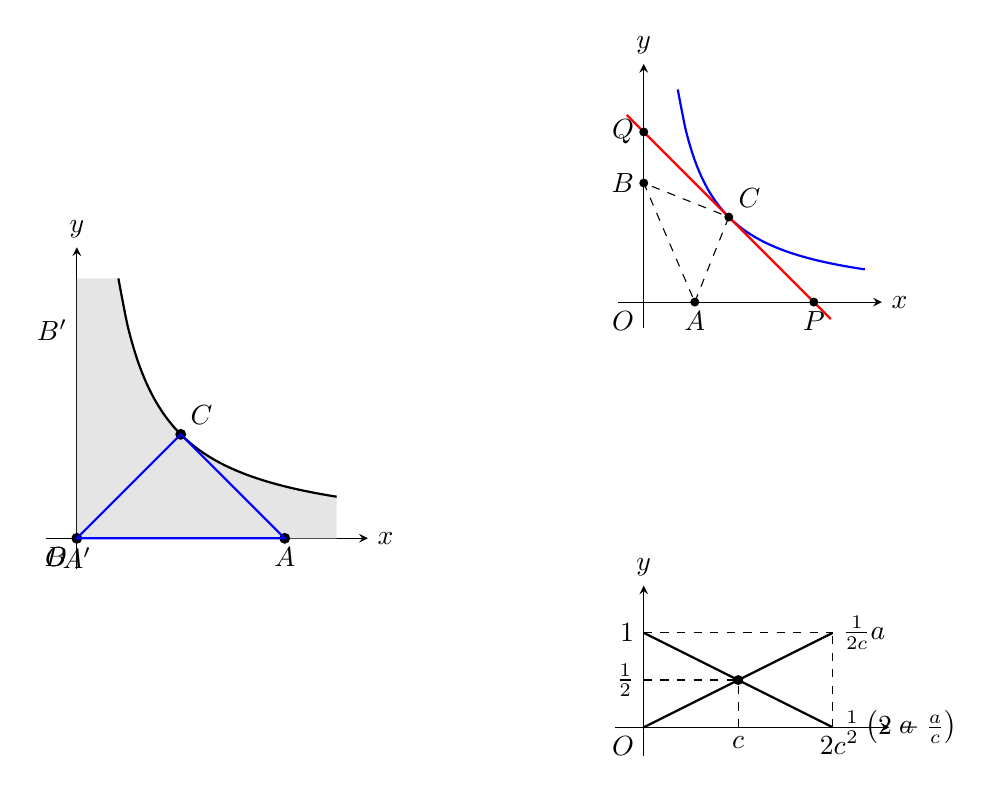
\begin{tikzpicture}[scale=1.2, >=stealth]
  % Upper Right Diagram: Tangent Line & Triangle
  \begin{scope}[shift={(6,2.5)}, scale=0.9]
    \draw[->] (-0.3,0) -- (2.8,0) node[right] {$x$};
    \draw[->] (0,-0.3) -- (0,2.8) node[above] {$y$};
    \node[below left] at (0,0) {$O$};
    \draw[domain=0.4:2.6, smooth, variable=\x, thick, blue] plot ({\x}, {1/\x});
    % Tangent line at c=1: y = -x + 2
    \draw[thick, red] (-0.2, 2.2) -- (2.2, -0.2);
    \fill (1,1) circle (1.5pt) node[above right] {$C$};
    \fill (2,0) circle (1.5pt) node[below] {$P$};
    \fill (0,2) circle (1.5pt) node[left] {$Q$};
    \fill (0.6,0) circle (1.5pt) node[below] {$A$};
    \fill (0,1.4) circle (1.5pt) node[left] {$B$};
    \draw[dashed] (0.6,0) -- (1,1) -- (0,1.4) -- cycle;
  \end{scope}

  % Middle Right Diagram: Graph of max S
  \begin{scope}[shift={(6,-2)}, scale=1.0]
    \draw[->] (-0.3,0) -- (2.6,0) node[right] {$a$};
    \draw[->] (0,-0.3) -- (0,1.5) node[above] {$y$};
    \node[below left] at (0,0) {$O$};
    \draw[thick] (0,0) -- (2,1) node[right] {$\frac{1}{2c}a$};
    \draw[thick] (0,1) -- (2,0) node[right] {$\frac{1}{2}\left(2-\frac{a}{c}\right)$};
    \draw[dashed] (1,0) node[below] {$c$} -- (1,0.5);
    \draw[dashed] (0,0.5) node[left] {$\frac{1}{2}$} -- (1,0.5);
    \fill (1,0.5) circle (1.5pt);
    \draw[dashed] (2,0) node[below] {$2c$} -- (2,1);
    \draw[dashed] (0,1) node[left] {$1$} -- (2,1);
  \end{scope}

  % Lower Left Diagram: Region D & Triangle
  \begin{scope}[shift={(0,0)}, scale=1.1]
    \draw[->] (-0.3,0) -- (2.8,0) node[right] {$x$};
    \draw[->] (0,-0.3) -- (0,2.8) node[above] {$y$};
    \node[below left] at (0,0) {$O$};
    % Shaded Region D
    \begin{scope}
      \clip (0,0) -- (2.5,0) -- (2.5,2.5) -- (0,2.5) -- cycle;
      \fill[gray!20] (0,0) -- (0,2.5) -- plot[domain=0.4:2.5, smooth] ({\x},{1/\x}) -- (2.5,0) -- cycle;
    \end{scope}
    \draw[domain=0.4:2.5, smooth, variable=\x, thick] plot ({\x}, {1/\x});
    \fill (1,1) circle (1.5pt) node[above right] {$C$};
    \fill (2,0) circle (1.5pt) node[below] {$A$};
    \fill (0,0) circle (1.5pt) node[below left] {$B$};
    \draw[thick, blue] (2,0) -- (0,0) -- (1,1) -- cycle;
    \node[left] at (0,2) {$B'$};
    \node[below] at (0,0) {$A'$};
  \end{scope}
\end{tikzpicture}
\end{center}

\noindent
[★以下, 解2]
$a$ を $0 \le a < c$, $a=c$, $c < a \le 2c$ で場合分けし, 各々の $\triangle ABC$ の高さの $\max$ をみる (以下略)。


\subsection*{第2問}

[解]
\[
P : \left(\frac{x}{2}\right)^2 + y^2 = 1, \quad Q : \left(\frac{x}{2}\right)^2 + \left(y - \frac{\sqrt{6}-\sqrt{2}}{2}\right)^2 = 1
\]
とおいて, $P, Q$ の囲む領域の面積が $M$ である。そこで次のような各点, $X = \frac{x}{2}, Y = y$ なる変換を行い, $P, Q$ を $P', Q'$ のように表す。
\[
P' : X^2 + Y^2 = 1, \quad Q' : X^2 + \left(Y - \frac{\sqrt{6}-\sqrt{2}}{2}\right)^2 = 1
\]
又, この変換で $M'$ の面積は $M$ の $\frac{1}{2}$ 倍にあたる $\dots$ ①

$S', T'$ は $\left(\mp \frac{\sqrt{6}+\sqrt{2}}{4}, \frac{\sqrt{6}-\sqrt{2}}{4}\right)$ だから, 図の $\theta$ は $\frac{\pi}{12}$ であり, したがって斜線部の面積 (対称性から $M'$ のそれの $\frac{1}{2}$ 倍) は,
\[
\frac{1}{2} (\pi - 2\theta) - 2 \cdot \frac{1}{2} \cdot \frac{\sqrt{6}+\sqrt{2}}{4} \cdot \frac{\sqrt{6}-\sqrt{2}}{4} = \frac{5}{12}\pi - \frac{1}{4}
\]
であり,
\[
(M \text{ の面積}) = 4 \cdot \left(\frac{5}{12}\pi - \frac{1}{4}\right) = \frac{5}{3}\pi - 1
\]
である。

\begin{center}
\begin{tikzpicture}[scale=1.5, >=stealth]
  % Original Ellipses Diagram
  \begin{scope}[shift={(-2.5,0)}]
    \draw[->] (-1.5,0) -- (1.5,0) node[right] {$x$};
    \draw[->] (0,-1.3) -- (0,1.8) node[above] {$y$};
    \draw[thick] (0,0) ellipse (1.2 and 0.8);
    \draw[thick] (0,0.5) ellipse (1.2 and 0.8);
    \begin{scope}
      \clip (0,0) ellipse (1.2 and 0.8);
      \fill[pattern=north east lines, pattern color=gray] (0,0.5) ellipse (1.2 and 0.8);
    \end{scope}
    \node at (-1.1,0.6) {$S$};
    \node at (1.1,0.6) {$T$};
  \end{scope}

  % Transformed Circles Diagram
  \begin{scope}[shift={(1.5,0)}]
    \draw[->] (-1.3,0) -- (1.3,0) node[right] {$X$};
    \draw[->] (0,-1.3) -- (0,1.8) node[above] {$Y$};
    \draw[thick] (0,0) circle (1.0);
    \draw[thick] (0,0.5) circle (1.0);
    \begin{scope}
      \clip (0,0) circle (1.0);
      \fill[pattern=north east lines, pattern color=gray] (0,0.5) circle (1.0);
    \end{scope}
    \draw (0,0) -- (0.966, 0.259) node[right] {$T'$};
    \draw (0,0) -- (-0.966, 0.259) node[left] {$S'$};
    \draw[dashed] (-0.966,0.259) -- (0.966,0.259);
    \draw (0.3,0) arc (0:15:0.3);
    \node at (0.45,0.08) {$\theta$};
    \node at (1.15,0.7) {$Q'$};
    \node at (1.15,-0.5) {$P'$};
  \end{scope}
\end{tikzpicture}
\end{center}

\noindent
[解2]
\[
\frac{S}{4} = \int_{0}^{\frac{\sqrt{6}+\sqrt{2}}{4}} \left( \sqrt{1 - X^2} - \frac{\sqrt{6}-\sqrt{2}}{4} \right) dX = \frac{5}{12}\pi - \frac{1}{4}
\]
\[
\therefore S = \frac{5}{3}\pi - 1
\]


\subsection*{第3問}

[解] $S_0$ は 2 ベクトル $\vec{p} = \begin{pmatrix} 0 - \frac{1}{2} \\ \frac{1}{2} - 0 \\ \frac{1}{2} - \left(-\frac{1}{2}\right) \end{pmatrix} = \frac{1}{2}\begin{pmatrix} -1 \\ 1 \\ 2 \end{pmatrix}$, $\vec{q} = \begin{pmatrix} 1 - 0 \\ 0 - \frac{1}{2} \\ 1 - \left(-\frac{1}{2}\right) \end{pmatrix} = \frac{1}{2}\begin{pmatrix} 2 \\ -1 \\ 3 \end{pmatrix}$ のはる平面と平行である。この法線ベクトルの 1 つに $\vec{n} = \begin{pmatrix} 1 \\ 1 \\ -1 \end{pmatrix}$ があるから, もとめる法線ベクトルは, $k \in \mathbb{R}$ として
\[
\vec{n_0} = k \begin{pmatrix} 1 \\ 1 \\ -1 \end{pmatrix}
\]
とおける。$|\vec{n_0}| = 1$ から $|3k^2| = 1 \implies k = \pm \frac{1}{\sqrt{3}}$ だから,
\[
\vec{n_0} = \pm \frac{1}{\sqrt{3}} \begin{pmatrix} 1 \\ 1 \\ -1 \end{pmatrix}
\]

(2)
$\vec{l}$ の方向ベクトル $\vec{l}' = \begin{pmatrix} 0 \\ 1 \\ 1 \end{pmatrix} - \begin{pmatrix} 1 \\ 0 \\ 0 \end{pmatrix} = \begin{pmatrix} -1 \\ 1 \\ 1 \end{pmatrix}$ とおく。$\vec{n_0}$ を $\vec{l}$ のまわりに回転した時に出来るベクトルが $\vec{n}$ である。$\vec{n_0}$ と $\vec{l}$ のなす角を $\theta$ とする。$\vec{n}$ と $\vec{l}$ のなす角も $\theta$ でひとしいので,
\[
\vec{n} \cdot \vec{l}' = |\vec{n}||\vec{l}'|\cos\theta = \sqrt{3}\cos\theta \quad \dots \text{①}
\]
又,
\[
\cos\theta = \frac{\vec{n_0} \cdot \vec{l}'}{|\vec{n_0}||\vec{l}'|} = \frac{\pm \frac{1}{\sqrt{3}} \begin{pmatrix} 1 \\ 1 \\ -1 \end{pmatrix} \cdot \begin{pmatrix} -1 \\ 1 \\ 1 \end{pmatrix}}{\sqrt{3}} = \frac{\mp 1}{3} \quad \dots \text{②}
\]
である。$\vec{n} = \begin{pmatrix} X \\ Y \\ Z \end{pmatrix}$ とおく。①, ②から
\[
-X + Y + Z = \pm \frac{1}{3} \quad \dots \text{③}
\]
又,
\[
X^2 + Y^2 + Z^2 = 1 \quad \dots \text{④}
\]
$Z \in \mathbb{R}$ から, $X^2 + Y^2 \le 1 \quad \dots \text{④}'$ である。③, ④'を満たす $(X, Y)$ を図示して右図太線部だから,
\[
-\frac{1+\sqrt{17}}{6} \le Y \le \frac{1+\sqrt{17}}{6}
\]
より, $\min |Y| = 0$, $\max |Y| = \frac{1+\sqrt{17}}{6}$.

[対称性から, 複号の片方について考えれば十分である。]

\begin{center}
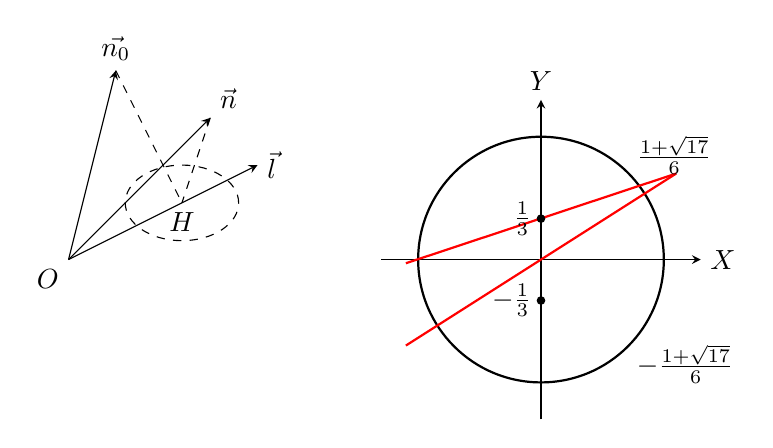
\begin{tikzpicture}[scale=1.2, >=stealth]
  % 3D rotation figure
  \begin{scope}[shift={(-2.5,0)}, scale=1.0]
    \draw[->] (0,0) -- (2,1) node[right] {$\vec{l}$};
    \draw[->] (0,0) -- (0.5,2) node[above] {$\vec{n_0}$};
    \draw[->] (0,0) -- (1.5,1.5) node[above right] {$\vec{n}$};
    \draw[dashed] (1.2, 0.6) circle (0.6 and 0.4);
    \draw[dashed] (0.5,2) -- (1.2,0.6);
    \draw[dashed] (1.5,1.5) -- (1.2,0.6) node[below] {$H$};
    \node[below left] at (0,0) {$O$};
  \end{scope}

  % 2D region in (X,Y) plane
  \begin{scope}[shift={(2.5,0)}, scale=1.3]
    \draw[->] (-1.3,0) -- (1.3,0) node[right] {$X$};
    \draw[->] (0,-1.3) -- (0,1.3) node[above] {$Y$};
    \draw[thick] (0,0) circle (1.0);
    \draw[thick, red] (-1.1, -0.7) -- (1.1, 0.7) node[right] {};
    \draw[thick, red] (-1.1, -0.03) -- (1.1, 0.7);
    \fill (0, 1/3) circle (1pt) node[left] {$\frac{1}{3}$};
    \fill (0, -1/3) circle (1pt) node[left] {$-\frac{1}{3}$};
    \node[right] at (0.7, 0.85) {$\frac{1+\sqrt{17}}{6}$};
    \node[right] at (0.7, -0.85) {$-\frac{1+\sqrt{17}}{6}$};
  \end{scope}
\end{tikzpicture}
\end{center}

\noindent
[解2] $\vec{OH} = \frac{\vec{n_0}\cdot\vec{l}'}{|\vec{l}'|^2}\vec{l}' = \frac{1}{3}\begin{pmatrix} 1 \\ -1 \\ -1 \end{pmatrix}$ より,
\[
\vec{HT} = \frac{1}{3}\begin{pmatrix} 1 \\ 1 \\ -1 \end{pmatrix} - \frac{1}{3}\begin{pmatrix} 1 \\ -1 \\ -1 \end{pmatrix} = \frac{1}{3}\begin{pmatrix} 0 \\ 2 \\ 0 \end{pmatrix}
\]
$\vec{HT}, \vec{l}'$ に垂直なベクトルのひとつを使って, コーシー・シュワルツの不等式より
\[
0 \le |y| \le \frac{1+\sqrt{17}}{6}
\]


\subsection*{第4問}

[解] (1) まず $a$ を固定する。$a > 0$ だから,
\[
\begin{cases}
\frac{2.7}{a} \le u \le \frac{3.3}{a} \\
\frac{4.5}{a} \le v \le \frac{5.4}{a}
\end{cases} \quad \dots \text{①}
\]
これを図示すると, 右のような長方形内部及び周になる。

次に, $0.9 \le a \le 1.1$ で $a$ を動かす。$A, B, C, D$ は
\[
A = \left( \frac{3.3}{a}, \frac{4.5}{a} \right), \quad B = \left( \frac{3.3}{a}, \frac{5.4}{a} \right), \quad C = \left( \frac{2.7}{a}, \frac{5.4}{a} \right), \quad D = \left( \frac{2.7}{a}, \frac{4.5}{a} \right)
\]
を動くので, 右図斜線部 (境界含む)。

\begin{center}
\begin{tikzpicture}[scale=1.2, >=stealth]
  % Rectangle for fixed a
  \begin{scope}[shift={(-2.5,0)}, scale=0.9]
    \draw[thick] (0,0) rectangle (2,1.2);
    \node[below left] at (0,0) {$D\left(\frac{2.7}{a}, \frac{4.5}{a}\right)$};
    \node[below right] at (2,0) {$A\left(\frac{3.3}{a}, \frac{4.5}{a}\right)$};
    \node[above right] at (2,1.2) {$B\left(\frac{3.3}{a}, \frac{5.4}{a}\right)$};
    \node[above left] at (0,1.2) {$C\left(\frac{2.7}{a}, \frac{5.4}{a}\right)$};
  \end{scope}

  % Region in uv-plane
  \begin{scope}[shift={(2.5,0)}, scale=1.1]
    \draw[->] (-0.3,0) -- (3.8,0) node[right] {$u$};
    \draw[->] (0,-0.3) -- (0,3.2) node[above] {$v$};
    \node[below left] at (0,0) {$0$};

    % Points
    % u_1 = 27/11 = 2.45, u_2 = 3, u_3 = 11/3 = 3.67
    % v_1 = 45/11 = 4.09, v_2 = 2*u, etc.
    \draw[dashed] (2.45,0) node[below] {$\frac{27}{11}$} -- (2.45,2.45);
    \draw[dashed] (3.0,0) node[below] {$3$} -- (3.0,2.7);
    \draw[dashed] (3.67,0) node[below] {$\frac{11}{3}$} -- (3.67,2.5);

    % Shaded region
    \fill[pattern=north east lines, pattern color=gray] (2.45, 2.05) -- (3.0, 2.7) -- (3.67, 2.7) -- (3.67, 2.25) -- (3.0, 1.8) -- (2.45, 1.8) -- cycle;
    \draw[thick] (2.45, 2.05) -- (3.0, 2.7) -- (3.67, 2.7) -- (3.67, 2.25) -- (3.0, 1.8) -- (2.45, 1.8) -- cycle;

    \draw (0,0) -- (3.5, 2.87) node[right] {$v = \frac{15}{11}u$};
    \draw (0,0) -- (1.5, 3.0) node[above] {$v = 2u$};
  \end{scope}
\end{tikzpicture}
\end{center}

(2) まず $Z$ の存在条件から, 判別式が 0 以上で,
\[
b^2 - ac \ge 0 \iff \left(\frac{b}{a}\right)^2 - \left(\frac{c}{a}\right) \ge 0 \quad (\because a > 0) \iff u^2 - v \ge 0 \quad \dots \text{①}
\]
この領域を $(u, v)$ が動く時, ①は常に満たされる。又,
\[
Z = \frac{b + \sqrt{b^2 - ac}}{a} = u + \sqrt{u^2 - v} \quad \dots \text{②}
\]
ここで, (1) の領域は, 式にすると,
\[
\begin{cases}
\frac{27}{11} \le u \le 3 \text{ の時, } \frac{45}{11} \le v \le 2u \\
3 \le u \le \frac{11}{3} \text{ の時, } \frac{15}{11}u \le v \le 6
\end{cases} \quad \dots \text{③}
\]
であることに注意すると, ②で $u$ を固定した時, $Z$ は $v$ の単調減少関数だから
\[
\begin{cases}
\frac{27}{11} \le u \le 3 \text{ の時, } \min Z = u + \sqrt{u^2 - 2u}, \quad \max Z = u + \sqrt{u^2 - \frac{45}{11}} \\
3 \le u \le \frac{11}{3} \text{ の時, } \min Z = u + \sqrt{u^2 - 6}, \quad \max Z = u + \sqrt{u^2 - \frac{15}{11}u}
\end{cases} \quad \dots \text{④}
\]
次に $u$ を動かす。

$1^\circ$ $\min Z$ について
$u$ の候補は, $u = \frac{27}{11}$ の時の $Z = \frac{27+3\sqrt{15}}{11}$ か, $u = 3$ の時の $Z = 3+\sqrt{3}$ である。前者の方が小さいので,
\[
\min Z = \frac{27+3\sqrt{15}}{11}
\]

$2^\circ$ $\max Z$ について
$u$ の候補は, $u = 3$ の時の $Z = 3+3\sqrt{\frac{2}{11}}$, $u = \frac{11}{3}$ の時の $Z = \frac{11+2\sqrt{19}}{3}$ である。後者の方が大きいので,
\[
\max Z = \frac{11+2\sqrt{19}}{3}
\]

以上から
\[
\begin{cases}
\min Z = \frac{3}{11}(9 + \sqrt{15}) \\
\max Z = \frac{1}{3}(11 + 2\sqrt{19})
\end{cases}
\]


\subsection*{第5問}

[解] 以下の解では, ゲームが終了する場合は含めないものとする。ただし, ちょうど終わる時は含む。

(1) $n$ 回じゃんけんして, 同じ手が出ているのは, ゲームが終了せず, かつ 2 人の勝ち数の合計が $k$ 回になっている時である。求める確率 $q$ は, $k \ge 2$ の時

$\text{i)} \ n < k \text{ の時}$
\[
q = 0
\]

$\text{ii)} \ n = k \text{ の時}$
$n$ 回とも引き分けがない時であるから,
\[
q = \left(1 - \frac{1}{3}\right)^n = \left(\frac{2}{3}\right)^n
\]

$\text{iii)} \ n > k \text{ の時}$
2 人の勝ちの合計が $k$ 回かつ, 片方が先に勝たなければ良い。ゆえに,
\begin{align*}
q &= {}_n\text{C}_k \left(\frac{2}{3}\right)^k \left(\frac{1}{3}\right)^{n-k} - 2 \cdot {}_{n-1}\text{C}_{k-1} \left(\frac{1}{3}\right)^k \left(\frac{1}{3}\right)^{n-k-1} \cdot \left(\frac{1}{3}\right) \\
&= {}_n\text{C}_k \left(\frac{1}{3}\right)^n \cdot 2^k - 2 \left(\frac{n-k}{n}\right) {}_n\text{C}_k \left(\frac{1}{3}\right)^n \\
&= 2 {}_n\text{C}_k \left(\frac{1}{3}\right)^n \left( 2^{k-1} - 1 + \frac{k}{n} \right)
\end{align*}
これをまとめて, $n < k$ の時 ${}_n\text{C}_k = 0$, 又, $k=1$ の時もこれで良いから,
\[
q = \frac{2}{3^n} {}_n\text{C}_k \left( 2^{k-1} - 1 + \frac{k}{n} \right)
\]

(2) $x, y$ は, $A, B$ の勝利回数を表す。ゆえに
\[
x + y \le n \quad \dots \text{①}
\]
又, $k$ 回までしか移動できないから,
\[
x, y \le k \quad \dots \text{②}
\]
このもとで考える。$n$ 回じゃんけんをしたということは, $n-1$ 回目までゲームは終了しなかったということだから, まず $x, y \le k-1$ の時,
\[
P(x, y) = {}_n\text{C}_x {}_{n-x}\text{C}_y \left(\frac{1}{3}\right)^x \left(\frac{1}{3}\right)^y \left(\frac{1}{3}\right)^{n-x-y} = {}_n\text{C}_x {}_{n-x}\text{C}_y \left(\frac{1}{3}\right)^n \quad \dots \text{③}
\]
$x = y = k$ となることはありえない (ゲームが終了している) ので, たとえば $x \le k-1, y = k$ の時, $B$ が最後に1勝しなければならないから,
\[
P(x, k) = {}_{n-1}\text{C}_{k-1} {}_{(n-1)-(k-1)}\text{C}_x \left(\frac{1}{3}\right)^n = {}_{n-1}\text{C}_{k-1} {}_{n-k}\text{C}_x \left(\frac{1}{3}\right)^n \quad (\text{①, ②から } k \le n)
\]
これは対称性により, $x = k, y \le k-1$ にも同じことが言える。よって ①, ②のもとで,
\[
P(x, y) = \begin{cases}
{}_n\text{C}_x {}_{n-x}\text{C}_y \left(\frac{1}{3}\right)^n & (x, y \le k-1) \\
{}_{n-1}\text{C}_{k-1} {}_{n-k}\text{C}_x \left(\frac{1}{3}\right)^n & (x \le k-1, y = k) \\
{}_{n-1}\text{C}_{k-1} {}_{n-k}\text{C}_y \left(\frac{1}{3}\right)^n & (y \le k-1, x = k) \\
0 & (\text{otherwise})
\end{cases}
\]

(3) $k = 2$ とする。(2) の $P(x, y)$ を用いて,
\begin{align*}
P &= \sum_{x, y \le 2} P(x, y) \\
&= P(0,0) + P(1,0) + P(0,1) + P(2,0) + P(1,1) + P(0,2) + P(2,1) + P(1,2) + P(2,2) \\
&= P(0,0) + 2 P(1,0) + 2 P(2,0) + P(1,1) + 2 P(2,1) + P(2,2) \\
&= \left(\frac{1}{3}\right)^n \left[ 1 + 2n + n(n-1) + n(n-1) + n(n-1)(n-2) + \frac{1}{4}n(n-1)(n-2)(n-3) \right] \\
&= \left(\frac{1}{3}\right)^n \frac{1}{4} \left[ n^4 - 2n^3 + 7n^2 + 2n + 4 \right] \quad \dots \text{④}
\end{align*}
一方 $n=3$ の時, 余事象を考えて,
\[
P = 1 - 2\left(\frac{1}{3}\right)^3 = \frac{25}{27}
\]
だから, $n=3$ でも ④は成立。以上から
\[
P = \frac{1}{4} \left(\frac{1}{3}\right)^n \left[ n^4 - 2n^3 + 7n^2 + 2n + 4 \right]
\]

\noindent
[* 問題文が悪い！ ゲーム終了の扱いをどうするのかが不明瞭。この解答では, 50年の解をとった。]


\subsection*{第6問}

[解] (1) 右図のように各点, 図形量をおく。
$\angle AOB = \frac{\pi}{2}$ から,
\[
x = \sqrt{2}\tan\left(\frac{\pi}{4} - \alpha\right) = \frac{1-m}{1+m}\sqrt{2}
\]
\[
AC = \sqrt{x^2+2} = \frac{2}{1+m}\sqrt{m^2+1}
\]
楕円の中心 $D$ は $AC$ の中点だから,
\[
AD = \frac{1}{2}AC = \frac{1}{1+m}\sqrt{m^2+1} \quad \dots \text{①}
\]
となる。したがって, $0 < \alpha < \pi/4$ の時
\[
l = AD \sin\alpha = \frac{\sqrt{m^2+1}}{1+m} \frac{m}{\sqrt{m^2+1}} = \frac{m}{1+m}
\]
となる。$D$ を通り $AB$ に平行な直線と軸の交点を $E$ とする。
\[
OE = 1 - l = \frac{1}{m+1}
\]
だから, $P$ を含み軸に垂直な平面での切り口は右図のような半径 $\frac{1}{m+1}$ の円である。
\[
DE = 1 - AD \cos\alpha = 1 - \frac{\sqrt{m^2+1}}{1+m}\frac{1}{\sqrt{1+m^2}} = \frac{m}{1+m} \quad (\because 0 < \alpha < \pi/2)
\]
だから
\[
DF = \sqrt{\left(\frac{1}{1+m}\right)^2 - \left(\frac{m}{1+m}\right)^2} = \frac{\sqrt{1-m^2}}{1+m} \quad \dots \text{②}
\]
①, ②のうち大きい方が $a$ であり,
\[
a = \frac{\sqrt{1+m^2}}{1+m}, \quad b = \frac{\sqrt{1-m^2}}{1+m}
\]

(2) 残った水の量が $\frac{1}{2} \cdot \left(\frac{1}{3}\pi\right) = \frac{1}{6}\pi$ だから,
\[
\frac{1}{6}\pi = \frac{1}{3}\pi a b h \quad \dots \text{③}
\]
ここで, $\triangle OAC$ の面積を2通りで表して,
\[
AC \cdot h = \sqrt{2} x
\]
\[
2\frac{\sqrt{1+m^2}}{1+m} \cdot h = \sqrt{2}\sqrt{2}\frac{1-m}{1+m} \implies h = \frac{1-m}{\sqrt{1+m^2}}
\]
だから, (1)とあわせて③に代入して
\[
\frac{1}{2} = \frac{\sqrt{1-m^2}}{(1+m)^2} (1-m)
\]
$1-m > 0$ から, 2乗して
\begin{align*}
(1+m)^4 &= 4(1-m)^2(1-m^2) \\
(1+m)^3 &= 4(1-m)^3 \\
1+m &= 2^{\frac{2}{3}}(1-m) \\
m &= \frac{2^{\frac{2}{3}}-1}{2^{\frac{2}{3}}+1}
\end{align*}

\begin{center}
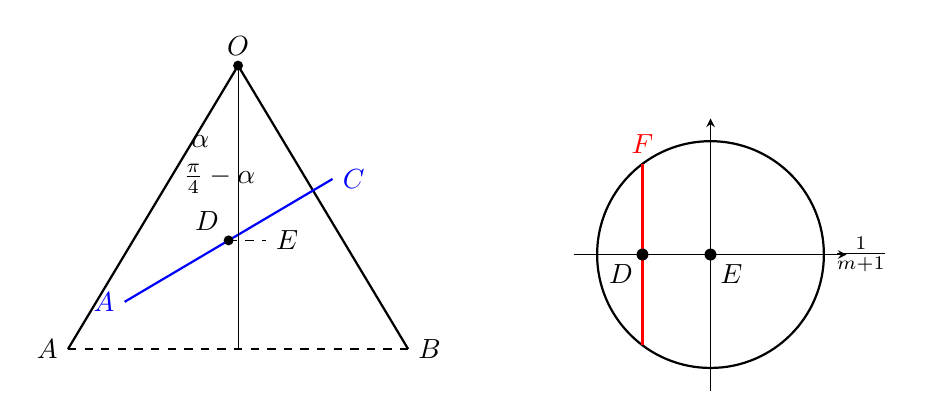
\begin{tikzpicture}[scale=1.2, >=stealth]
  % Cone cross section
  \begin{scope}[shift={(-2.5,0)}, scale=1.0]
    \draw[thick] (0,2) -- (-1.8,-1) node[left] {$A$};
    \draw[thick] (0,2) -- (1.8,-1) node[right] {$B$};
    \draw[dashed] (-1.8,-1) -- (1.8,-1);
    \draw[thick, blue] (-1.2,-0.5) node[left] {$A$} -- (1.0, 0.8) node[right] {$C$};
    \fill (0,2) circle (1.5pt) node[above] {$O$};
    \fill (-0.1, 0.15) circle (1.5pt) node[above left] {$D$};
    \draw (0,2) -- (0,-1);
    \draw[dashed] (-0.1, 0.15) -- (0.3, 0.15) node[right] {$E$};
    \node at (-0.4, 1.2) {$\alpha$};
    \node at (-0.2, 0.8) {$\frac{\pi}{4}-\alpha$};
  \end{scope}

  % Circular cross section
  \begin{scope}[shift={(2.5,0)}, scale=1.2]
    \draw[thick] (0,0) circle (1.0);
    \draw[->] (-1.2,0) -- (1.2,0);
    \draw[->] (0,-1.2) -- (0,1.2);
    \draw[thick, red] (-0.6, -0.8) -- (-0.6, 0.8) node[above] {$F$};
    \fill (-0.6,0) circle (1.5pt) node[below left] {$D$};
    \fill (0,0) circle (1.5pt) node[below right] {$E$};
    \node[right] at (1.0, 0) {$\frac{1}{m+1}$};
  \end{scope}
\end{tikzpicture}
\end{center}

\noindent
[解2]
(1) $O$ を原点, 新たな水面が $xz$ 平面と平行になるように, $xyz$ 空間をおく。$\triangle OAB$ が $xz$ 平面にあるようにした。この時, 軸の方向ベクトル $\vec{l}$ は,
\[
\vec{l} = \begin{pmatrix} \cos(\pi/2+\alpha) \\ 0 \\ \sin(\pi/2+\alpha) \end{pmatrix} = \begin{pmatrix} -\sin\alpha \\ 0 \\ \cos\alpha \end{pmatrix} = \frac{1}{\sqrt{m^2+1}}\begin{pmatrix} -m \\ 0 \\ 1 \end{pmatrix}
\]
である。円錐側面上の点 $P(X, Y, Z)$ について, $\vec{OP} \cdot \vec{l} = |\vec{OP}| \cos \frac{\pi}{4}$ だから,
\[
(-mX + Z) = \sqrt{X^2 + Y^2 + Z^2} \sqrt{m^2+1} \frac{1}{\sqrt{2}}
\]
両辺2乗して,
\[
\frac{1-m^2}{2}Z^2 = \frac{1-m^2}{2}X^2 + 2mZX + \frac{1+m^2}{2}Y^2 \quad \dots \text{①}
\]
水面は $Z = \frac{1-m}{\sqrt{1+m^2}}$ だから, ①に代入して整理すると, 中心が $D'\left(-\frac{2m}{(1+m)\sqrt{1+m^2}}, 0\right)$, 長半径, 短半径が
\[
a = \frac{\sqrt{1+m^2}}{1+m}, \quad b = \frac{\sqrt{1-m^2}}{1+m}
\]
の楕円である。中心と平面 $AB$ の距離が $h = \frac{1-m}{\sqrt{1+m^2}}$ である。

\end{document}
